\hypertarget{modelling-reactive-behavior-notation---mode-control}{%
\section{Modelling Reactive Behavior Notation -
Mode-Control}\label{modelling-reactive-behavior-notation---mode-control}}

\begin{itemize}
\tightlist
\item
  Mode-Control is defined within a cluster Reactive System
\item
  Mode-Control is one of three synchronous interaction mechanisms
  between reactive objects
\end{itemize}

\hypertarget{application}{%
\subsection{Application}\label{application}}

\begin{itemize}
\tightlist
\item
  One state-diagram for each mode
\item
  Each reactive-object has 1-n modes
\item
  All modes together define the state-machine of a reactive object
\item
  With mode control you can simplify the state diagrams and insert mode
  settings
\item
  There are two different modes ``working'' and ``shutdown'' in the
  example
\item
  if you are in the state ``Draining'' and the event ``evEmptied'' is
  fired, it depends on the mode which flow is happening now
\item
  If you are in ``working'', it goes to ``Filling''
\item
  If you are in ``shutdown'', it goes to ``Idle''
\end{itemize}

\begin{figure}[H]
\centering
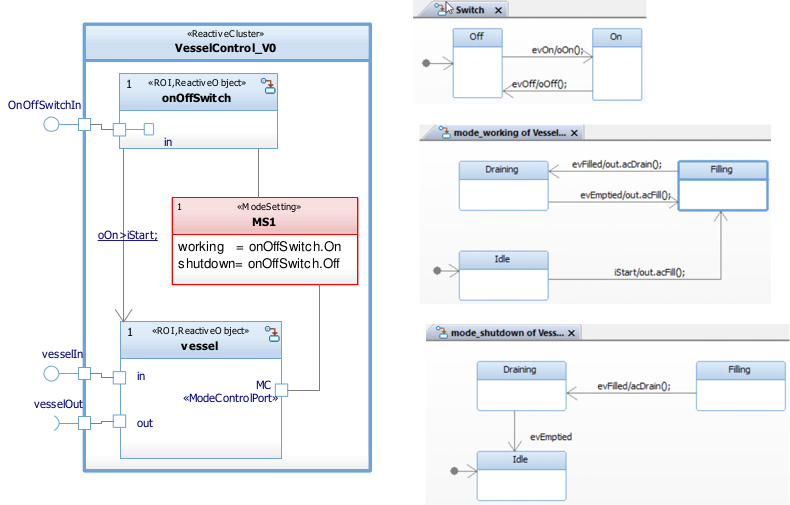
\includegraphics[width=0.85\textwidth]{figures/modecontrolCiro.png}
\caption{Mode Control Example}
\end{figure}

\clearpage
\hypertarget{mode-control-connection}{%
\subsection{Mode-Control-Connection}\label{mode-control-connection}}

\begin{itemize}
\tightlist
\item
  Belongs to the cluster
\item
  1-n masters
\item
  1 slave
\item
  Mode-Setting: a logical expression, - based on master-states is
  assigned to each mode
\end{itemize}

Example: \{modeX = masterA.on \& masterB.running modeY = masterA.off \&
masterB.running modeZ = !masterB.running\}

\hypertarget{mode-control-interaction}{%
\subsection{Mode-Control-Interaction}\label{mode-control-interaction}}

\begin{itemize}
\tightlist
\item
  Initial mode is indirectly determined by the initial state of each
  master
\item
  Nevertheless, there must be an initial state defined for each mode
\item
  Mode-control-interaction is initiated if a slave-object is activated
  by a trigger (event-message or in-pulse) in the same way as with
  state-inspection
\item
  A mode change doesn't initiate a state change by the slave
\item
  If a slave receives an in-pulse immediately after a mode-change, this
  in-pulse is handled in the new mode
\item
  Sequence of a reactive-object-step (reaction to trigger):
  \begin{itemize}
      \item ModeSelection()
      \item GateEvaluation()
      \item StateTransition()
      \item OutputMessageGeneration()
      \item OutpulseGeneration()
  \end{itemize}
\end{itemize}

\clearpage